\documentclass[a4paper]{article}
\usepackage[T1]{fontenc}			% \chapter package
\usepackage[italian]{babel}
\usepackage[italian]{isodate}  		% date format
\usepackage{graphicx}				% manage images
\usepackage{amsfonts}
\usepackage{booktabs}				% high quality tables
\usepackage{amsmath}				% math package
\usepackage{amssymb}				% another math package (e.g. \nexists)
\usepackage{bm}                     % bold math symbols
\usepackage{mathtools}				% emphasize equations
\usepackage{stmaryrd} 				% '\llbracket' and '\rrbracket'
\usepackage{amsthm}					% better theorems
\usepackage{enumitem}				% manage list
\usepackage{pifont}					% nice itemize
\usepackage{cancel}					% cancel math equations
\usepackage{caption}				% custom caption
\usepackage[]{mdframed}				% box text
\usepackage{multirow}				% more lines in a table
\usepackage{textcomp, gensymb}		% degree symbol
\usepackage[x11names]{xcolor}		% RGB color
\usepackage[many]{tcolorbox}				% colorful box
\usepackage{multicol}				% more rows in a table (used for the lists)
\usepackage{listings}
\usepackage{url}
\usepackage{qrcode}
\usepackage{fontawesome5}
\usepackage{ragged2e}
\usepackage{cite}                   % references
\usepackage{imakeidx}               % index
\makeindex[program=makeindex, columns=1,
           title=Index, 
           intoc,
           options={-s index-style.ist}]


\definecolor{codegreen}{rgb}{0,0.6,0}
\definecolor{codegray}{rgb}{0.5,0.5,0.5}
\definecolor{codepurple}{rgb}{0.58,0,0.82}
\definecolor{backcolour}{rgb}{0.95,0.95,0.92}
\lstdefinestyle{mystyle}{
    backgroundcolor=\color{backcolour},   
    commentstyle=\color{codegreen},
    keywordstyle=\color{magenta},
    numberstyle=\tiny\color{codegray},
    stringstyle=\color{codepurple},
    basicstyle=\ttfamily\footnotesize,
    breakatwhitespace=false,         
    breaklines=true,                 
    captionpos=b,                    
    keepspaces=true,                 
    numbers=left,                    
    numbersep=5pt,                  
    showspaces=false,                
    showstringspaces=false,
    showtabs=false,                  
    tabsize=2
}
\lstset{style=mystyle}


% draw a frame around given text
\newcommand{\framedtext}[1]{%
	\par%
	\noindent\fbox{%
		\parbox{\dimexpr\linewidth-2\fboxsep-2\fboxrule}{#1}%
	}%
}


% table of content links
\usepackage{xcolor}
\usepackage[linkcolor=black, citecolor=blue, urlcolor=cyan]{hyperref} % hypertexnames=false
\hypersetup{
	colorlinks=true
}


\newtheorem{theorem}{\textcolor{Red3}{\underline{Theorem}}}
\renewcommand{\qedsymbol}{QED}
\newcommand{\dquotes}[1]{``#1''}
\newcommand{\longline}{\noindent\rule{\textwidth}{0.4pt}}
\newcommand{\circledtext}[1]{\raisebox{.5pt}{\textcircled{\raisebox{-.9pt}{#1}}}}
\newcommand{\definition}[1]{\textcolor{Red3}{\textbf{#1}}\index{#1}}
\newcommand{\example}[1]{\textcolor{Green4}{\textbf{#1}}}
\newcommand{\highspace}{\vspace{1.2em}\noindent}
\newenvironment{rowequmat}[1]{\left(\array{@{}#1@{}}}{\endarray\right)}
\newenvironment{rowequmatbra}[1]{\left[\array{@{}#1@{}}}{\endarray\right]}

\begin{document}
    \newcounter{definition}[section]
    \newcounter{example}[section]
    
    \newtcolorbox[use counter = definition]{definitionbox}[1][]{%
        colback=red!5!white,
        colframe=red!75!black,
        fonttitle=\bfseries,
        title={Definizione \thetcbcounter #1} %
    }
    
    \newtcolorbox[use counter = example]{examplebox}[1][]{%
        breakable,
        enhanced,
        colback=Green4!5!white,
        colframe=Green4!75!black,
        fonttitle=\bfseries,
        title={Esempio \thetcbcounter #1} %
    }

    %%%%%%%%%%%%%%%
    % Notes cover %
    %%%%%%%%%%%%%%%
    \author{260236}
\title{Software Engineering for HPC - Notes}
\date{\printdayoff\today}
\maketitle

    %%%%%%%%%%%
    % Preface %
    %%%%%%%%%%%
	\section*{Preface}

Every theory section in these notes has been taken from two sources:
\begin{itemize}
    \item None
\end{itemize}
About:
\begin{itemize}
    \item[\faIcon{github}] \href{https://github.com/PoliMI-HPC-E-notes-projects-AndreVale69/HPC-E-PoliMI-university-notes}{GitHub repository}
\end{itemize}

    %%%%%%%%%%%%%%%%%%%%%
    % Table of contents %
    %%%%%%%%%%%%%%%%%%%%%
    \tableofcontents

    %%%%%%%%%%%%%%%%%%%%%%%%%
    % Equazioni non lineari %
    %%%%%%%%%%%%%%%%%%%%%%%%%
    \section{Equazioni non lineari}

\subsection{Introduzione}

Il \textbf{calcolo degli zeri di una funzione} $f$ reale di variabile reale o delle \textbf{radici dell'equazione} $f\left(x\right)=0$, è un problema assai ricorrente nel Calcolo Scientifico.

\highspace
In generale, \emph{non è possibile} approntare metodi numerici che calcolino gli zeri di una generica funzione in un numero finito di passi. I metodi numerici per la risoluzione di questo problema sono pertanto necessariamente \emph{iterativi}. A partire da uno o più dati iniziali, scelti convenientemente, essi generano una successione di valori $x^{\left(k\right)}$ che, sotto opportune ipotesi, convergerà ad uno zero $\alpha$ della funzione $f$ studiata.

\longline

\subsection{Il metodo di bisezione (o iterativo)}

Sia $f$ una funzione continua in $\left[a,b\right]$ tale che $f\left(a\right)f\left(b\right) < 0$. Per cui, vale il \href{https://www.youmath.it/lezioni/analisi-matematica/limiti-continuita-e-asintoti/723-teorema-degli-zeri.html}{teorema degli zeri di una funzione continua}, ossia $f$ ammette almeno uno zero in $\left(a,b\right)$.

\highspace
Si supponga che ci sia un solo zero, indicato con $\alpha$ e nel caso in cui ce ne sia più di uno, individuare un intervallo tale che ne contenga solo uno.

\highspace
Il \definition{metodo di bisezione} (o \textbf{iterativo}\index{metodo iterativo}) è una strategia che si suddivide nei seguenti passaggi:
\begin{enumerate}
    \item \textbf{Dimezzare l'intervallo di partenza};
    \item \textbf{Selezionare tra i due sotto-intervalli ottenuti quello nel quale} $f$ \textbf{cambia di segno agli estremi};
    \item \textbf{Applicare ricorsivamente questa procedura all'ultimo intervallo selezionato}.
\end{enumerate}

\highspace
Matematicamente parlando, dato $I^{(0)} = \left(a,b\right)$, e più in generale, $I^{(k)}$ il sotto-intervallo selezionato al passo $k$-esimo, si sceglie come $I^{\left(k+1\right)}$ il semi-intervallo di $I^{(k)}$ ai cui estremi $f$ cambia di segno.

\highspace
Questa procedura garantisce che ogni sotto-intervallo selezionato $I^{(k)}$ conterrà $\alpha$. Questo poiché la successione $\left\{x^{(k)}\right\}$ dei punti medi dei sotto-intervalli $I^{(k)}$ dovrà ineluttabilmente convergere a $\alpha$, in quanto la \textbf{lunghezza dei sotto-intervalli tende a} $0$ per $k$ che \textbf{tende all'infinito}.

\newpage

\noindent
Formalizziamo questa idea con un piccolo algoritmo. Ponendo:
\begin{equation*}
    a^{(0)} = a, \hspace{1em} b^{(0)} = b, \hspace{1em} I^{(0)} = \left(a^{(0)}, b^{(0)}\right), \hspace{1em} x^{(0)} = \dfrac{a^{(0)} + b^{(0)}}{2}
\end{equation*}
Al passo $k \ge 1$ il metodo di bisezione calcolerà il semi-intervallo $I^{(k)} = \left(a^{(k)}, b^{(k)}\right)$ dell'intervallo $I^{(k-1)} = \left(a^{\left(k-1\right)}, b^{\left(k-1\right)}\right)$, nel seguente modo (si ricorda che $\alpha$ è lo zero che si sta cercando):
\begin{enumerate}
    \item Calcolo $x^{\left(k-1\right)} = \dfrac{a^{\left(k-1\right)} + b^{\left(k-1\right)}}{2}$

    \item Se $f\left(x^{\left(k-1\right)}\right) = 0$:
    \begin{enumerate}
        \item Allora $\alpha = x^{\left(k-1\right)}$ e l'algoritmo \underline{termina}.
    \end{enumerate}
    
    \item Altrimenti, se $f\left(a^{\left(k-1\right)}\right) \cdot f\left(x^{\left(k-1\right)}\right) < 0$:
    \begin{enumerate}
        \item Si pone $a^{(k)} = a^{\left(k-1\right)}$
        \item Si pone $b^{(k)} = x^{\left(k-1\right)}$
        \item Si incrementa $k+1$ e si \underline{ripete ricorsivamente}.
    \end{enumerate}
    
    \item Altrimenti, se $f\left(x^{\left(k-1\right)}\right) \cdot f\left(b^{\left(k-1\right)}\right) < 0$:
    \begin{enumerate}
        \item Si pone $a^{(k)} = x^{\left(k-1\right)}$
        \item Si pone $b^{(k)} = b^{\left(k-1\right)}$
        \item Si incrementa $k+1$ e si \underline{ripete ricorsivamente}.
    \end{enumerate}
\end{enumerate}

\begin{examplebox}
    Data la funzione $f\left(x\right) = x^{2} - 1$, si parta da $a^{(0)} = -0.25$ e $b^{(0)} = 1.25$, e si applichi il metodo di bisezione:
    \begin{enumerate}
        \item Con $a^{(0)} = -0.25$ e $b^{(0)} = 1.25$:
        \begin{enumerate}
            \item Si calcola il punto medio:
            \begin{equation*}
                x^{(0)} = \dfrac{a^{(0)} + b^{(0)}}{2} = \dfrac{-0.25 + 1.25}{2} = 0.5
            \end{equation*}

            \item Si calcola la funzione con il punto medio come parametro:
            \begin{equation*}
                f\left(0.5\right) = 0.5^{2} - 1 = -0.75
            \end{equation*}

            \item Dato che la funzione nel punto medio non è uguale a zero, l'algoritmo deve continuare. Per farlo, bisogna sostituire il punto medio con uno dei due estremi. Per decidere quale dei due sostituire, è necessario capire in quale cambia valore la funzione. Si verifica inizialmente con $a^{(0)}$:
            \begin{equation*}
                \begin{array}{rcl}
                    f\left(a^{(0)}\right)f\left(x^{(0)}\right) < 0 &=& f\left(-0.25\right)f\left(0.5\right) < 0 \\ [.5em]
                    &=& \left(-0.9375 \cdot -0.75\right) < 0 \\ [.5em]
                    &=& 0.703125 \text{ \ding{55}}
                \end{array}
            \end{equation*}
            
            \item Si procede con l'algoritmo, provando adesso la $b^{(0)}$:
            \begin{equation*}
                \begin{array}{rcl}
                    f\left(x^{(0)}\right)f\left(b^{(0)}\right) < 0 &=& f\left(0.5\right)f\left(1.25\right) < 0 \\ [.5em]
                    &=& \left(-0.75 \cdot 0.5625\right) < 0 \\ [.5em]
                    &=& -0.421875 \text{ \ding{51}}
                \end{array}
            \end{equation*}

            \item Si pone $a^{(1)} = x^{(0)} = 0.5$

            \item Si pone $b^{(1)} = b^{(0)} = 1.25$

            \item Si incrementa $k$, $k = k + 1 = 0 + 1 = 1$
        \end{enumerate}

        \item Con $a^{(1)} = 0.5$ e $b^{(1)} = 1.25$:
        \begin{enumerate}
            \item Si calcola il punto medio:
            \begin{equation*}
                x^{(1)} = \dfrac{a^{(1)} + b^{(1)}}{2} = \dfrac{0.5 + 1.25}{2} = 0.875
            \end{equation*}

            \item Si calcola la funzione con il punto medio come parametro:
            \begin{equation*}
                f\left(0.875\right) = 0.875^{2} - 1 = -0.234375
            \end{equation*}

            \item Dato che la funzione nel punto medio non è uguale a zero, l'algoritmo deve continuare:
            \begin{equation*}
                \begin{array}{rcl}
                    f\left(a^{(1)}\right)f\left(x^{(1)}\right) < 0 &=& f\left(0.5\right)f\left(-0.234375\right) < 0 \\ [.5em]
                    &=& \left(-0.75 \cdot -0.945068359375\right) < 0 \\ [.5em]
                    &=& 0.70880126953125 \text{ \ding{55}}
                \end{array}
            \end{equation*}
            
            \item Si procede con l'algoritmo:
            \begin{equation*}
                \begin{array}{rcl}
                    f\left(x^{(1)}\right)f\left(b^{(1)}\right) < 0 &=& f\left(-0.234375\right)f\left(1.25\right) < 0 \\ [.5em]
                    &=& \left(-0.945068359375 \cdot 0.5625\right) < 0 \\ [.5em]
                    &=& -0.5316009521484375 \text{ \ding{51}}
                \end{array}
            \end{equation*}

            \item Si pone $a^{(2)} = x^{(1)} = 0.875$

            \item Si pone $b^{(2)} = b^{(1)} = 1.25$

            \item Si incrementa $k$, $k = k + 1 = 1 + 1 = 2$
        \end{enumerate}
    \end{enumerate}
    Si omettono i restanti calcoli per $k=2, k=3$, ma si lasciano qua di seguito i risultati:
    \begin{itemize}
        \item $I^{(2)} = \left(0.875, 1.25\right)$ e $x^{(2)} = 1.0625$
        \item $I^{(3)} = \left(0.875, 1.0625\right)$ e $x^{(2)} = 0.96875$
    \end{itemize}

    \newpage

    \noindent
    Nella seguente figura si possono vedere le iterazioni effettuate:
    \begin{center}
        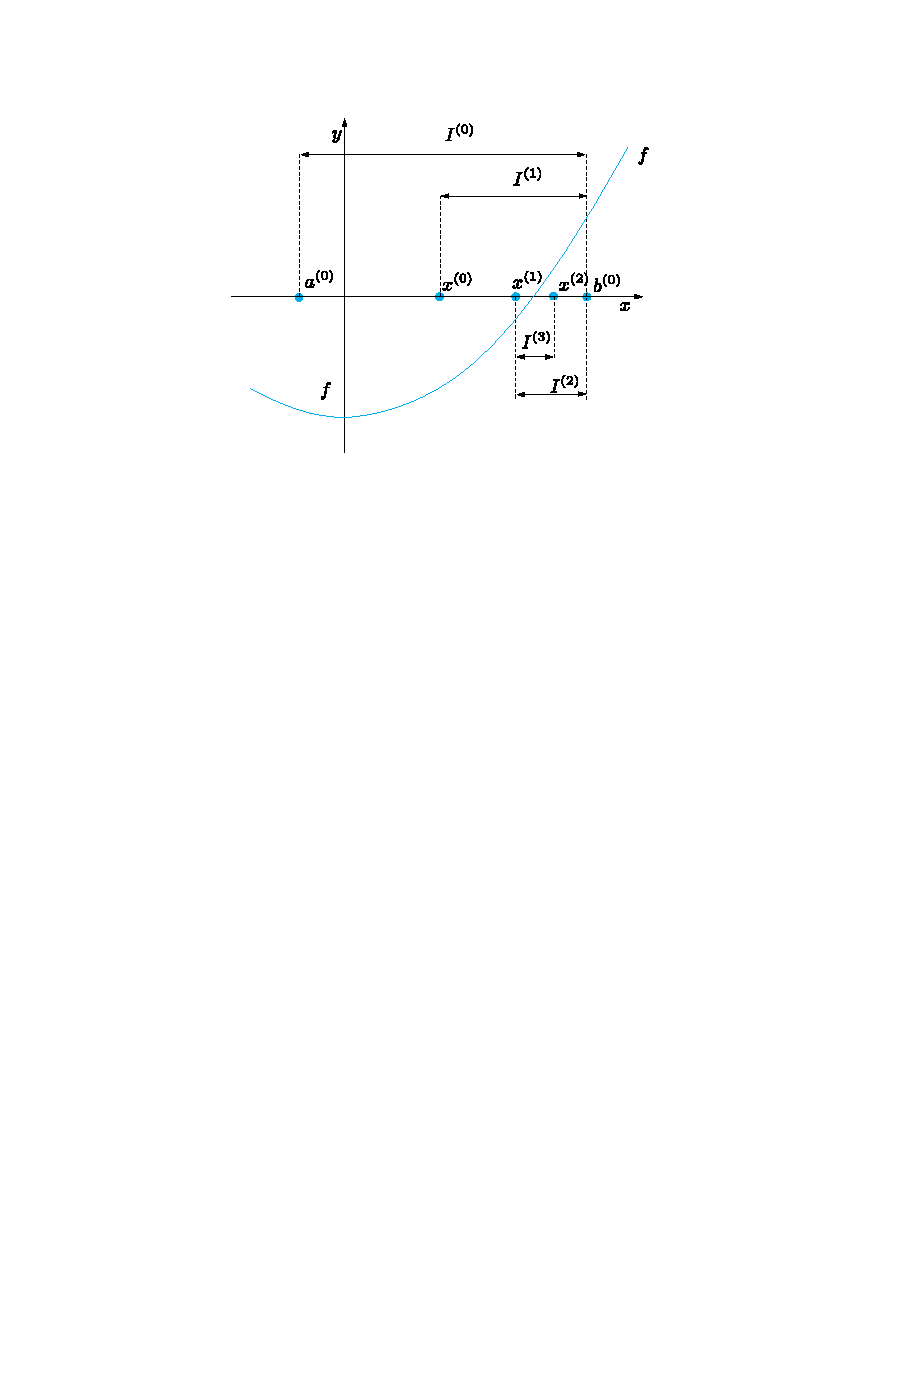
\includegraphics[width=.7\textwidth]{img/metodo-di-bisezione-1.pdf}
        \captionof*{figure}{Iterazioni effettuate.\cite{quarteroni2017calcolo}}
    \end{center}
    
    \noindent
    Si noti che ogni intervallo $I^{(k)}$ contiene lo zero $\alpha$. Inoltre, la successione $\left\{x^{(k)}\right\}$ converge necessariamente allo zero $\alpha$ in quanto ad ogni passo l'ampiezza $\left| I^{(k)} \right| = b^{(k)} - a^{(k)}$ dell'intervallo $I^{(k)}$ si dimezza.
\end{examplebox}

\noindent
Il valore $I^{(k)}$ può essere riassunto come:
\begin{equation*}
    \left|I^{(k)}\right| = \left(\dfrac{1}{2}\right)^{k} \cdot \left| I^{(0)} \right|
\end{equation*}
E di conseguenza l'\textbf{errore al passo} $\bm{k}$ può essere calcolato come:
\begin{equation*}
    \left| e^{(k)} \right| = \left| x^{(k)} - \alpha \right| < \dfrac{1}{2} \cdot \left| I^{(k)} \right| = \left(\dfrac{1}{2}\right)^{k+1} \cdot \left(b-a\right)
\end{equation*}
Inoltre, data una certa \textbf{tolleranza} $\varepsilon$, per \textbf{garantire che l'errore al passo $k$ sia minore della tolleranza data} (ovvero, $\left| e^{(k)} \right| < \varepsilon$), basta applicare la seguente formula:
\begin{equation}
    k_{\min} > \log_{2} \left(\dfrac{b-a}{\varepsilon}\right) - 1
\end{equation}
Dove $k_{\min}$ rappresenta il \textbf{numero \underline{minimo} di iterazioni prima di trovare un intero che soddisfi la disuguaglianza}.

\begin{flushleft}
    \textcolor{Red2}{\faIcon{exclamation-triangle} \textbf{Possibile svantaggio}}
\end{flushleft}
Il metodo di bisezione \textbf{non garantisce una riduzione monotona dell'errore}, ma solo il dimezzamento dell'ampiezza dell'intervallo all'interno del quale si cerca lo zero. Infatti, \textbf{non viene tenuto conto del reale andamento di} $f$ e questo può provocare il mancato coinvolgimento di approssimazioni di $\alpha$ accurate.
    \subsection{Il metodo di Newton}

Il \definition{metodo di Newton} sfrutta la funzione $f$ maggiormente rispetto al metodo di bisezione, usando i suoi valori e la sua derivata.

\highspace
Si ricorda che la retta tangente alla curva $\left(x, f\left(x\right)\right)$ nel punto $x^{(k)}$ è:
\begin{equation*}
    y\left(x\right) = f\left(x^{(k)}\right) + f'\left(x^{(k)}\right)\left(x-x^{(k)}\right)
\end{equation*}
\textbf{Cercando} un $x^{\left(k+1\right)}$ tale che la \textbf{retta tangente in quel punto sia uguale a zero} $y\left(x^{\left(k+1\right)}\right) = 0$, allora si trova:
\begin{equation}\label{eq: metodo di Newton}
    x^{\left(k+1\right)} = x^{\left(k\right)} - \dfrac{f\left(x^{\left(k\right)}\right)}{f'\left(x^{\left(k\right)}\right)} \hspace{2em} k \ge 0
\end{equation}
Purché la derivata prima nel punto $x^{(k)}$ sia diversa da zero, cioè $f'\left(x^{k}\right) \ne 0$.

\highspace
Questa equazione consente di calcolare una successione di valori $x^{(k)}$ a partire da un dato iniziale $x^{(0)}$. In altre parole, il \textbf{metodo di Newton calcola lo zero di $f$ sostituendo localmente a $f$ la sua retta tangente}.

\highspace
A differenza del metodo di bisezione, tale \textbf{metodo converge allo zero in un solo passo quando la funzione $f$ è lineare}, ovvero nella forma $f\left(x\right) = a_{1}x + a_{0}$.

\begin{flushleft}
    \textcolor{Red2}{\faIcon{exclamation-triangle} \textbf{Limitazione}}
\end{flushleft}
La \textbf{convergenza} del metodo di Newton \underline{non} è garantita \textbf{per ogni scelta} di $x^{(0)}$, ma \textbf{soltanto} per valori di $x^{(0)}$ \textbf{sufficientemente vicini} ad $\alpha$, ovvero \textbf{appartenenti ad un intorno} $I\left(\alpha\right)$ sufficientemente piccolo di $\alpha$.

\highspace
Alcune osservazioni a seguito anche di questa limitazione:
\begin{itemize}
    \item A seguito di questa limitazione, risulta evidente che se $x^{(0)}$ è stato scelto opportunamente e se lo zero $\alpha$ è semplice ($f'\left(\alpha\right) \ne 0$), allora il metodo converge.
    
    \item Nel caso in cui $f$ è derivabile con continuità pari a due, allora si ottiene la seguente convergenza:
    \begin{equation}
        \displaystyle \lim_{k \rightarrow \infty} \dfrac{x^{\left(k+1\right) - \alpha}}{\left(x^{(k)} - \alpha\right)^{2}} = \dfrac{f''\left(\alpha\right)}{2f'\left(\alpha\right)}
    \end{equation}
    Il significato è: se $f'\left(\alpha\right) \ne 0$ il metodo di Newton converge almeno quadraticamente o con \textbf{ordine 2}.

    In parole povere, \textbf{per $k$ sufficientemente grande, l'errore al passo $\left(k+1\right)$-esimo si comporta come il quadrato dell'errore al passo $k$-esimo, moltiplicato per una costante indipendente da $k$}.

    \item Se lo zero $\alpha$ ha molteplicità $m$ maggiore di $1$, ovverosia:
    \begin{equation*}
        f'\left(\alpha\right) = 0, \dots, f^{\left(m-1\right)}\left(\alpha\right) = 0
    \end{equation*}
    Allora il metodo di Newton è ancora convergente, purché $x^{(0)}$ sia scelto opportunamente e $f'\left(x\right) \ne 0$ $\forall x \in I\left(\alpha\right) \setminus \left\{\alpha\right\}$. Tuttavia in questo caso l'ordine di convergenza è pari a 1. In tal caso, l'ordine 2 può essere ancora recuperato usando la seguente relazione al posto dell'equazione~\ref{eq: metodo di Newton} ufficiale:
    \begin{equation}
        x^{\left(k+1\right)} = x^{(k)} - m \cdot \dfrac{f\left(x^{(k)}\right)}{f'\left(x^{(k)}\right)} \hspace{2em} k \ge 0
    \end{equation}
    Purché $f'\left(x^{(k)}\right) \ne 0$. Naturalmente, questo \textbf{metodo di Newton modificato} richiede una conoscenza a priori di $m$.
\end{itemize}

\longline

\subsubsection{Come arrestare il metodo di Newton}

Data una tolleranza fissa $\varepsilon$, esistono due tecniche applicabili per capire quando è necessario fermarsi ed evitare di continuare ad iterare:
\begin{itemize}
    \item La \definition{differenza fra due iterate consecutive}, il quale si arresta in corrispondenza del più piccolo intero $k_{\min}$ per il quale:
    \begin{equation}
        \left| x^{\left(k_{\min}\right)} - x^{\left(k_{\min} - 1\right)} \right| < \varepsilon
    \end{equation}
    (test sull'incremento).

    \item Un'altra tecnica applicata anche per altri metodi iterativi è il \definition{residuo} al passo $k$, il quale è definito come:
    \begin{equation*}
        r^{(k)} = f\left(x^{(k)}\right)
    \end{equation*}
    Che è nullo quando $x^{(k)}$ è uno zero di $f$. In questo modo, il metodo viene arrestato alla prima iterata $k_{\min}$:
    \begin{equation}
        \left| r^{\left(k_{\min}\right)} \right| = \left| f\left(x^{\left(k_{\min}\right)}\right) \right| < \varepsilon
    \end{equation}
    Da notare che tale tecnica fornisce una \textbf{stima accurata dell'errore} \underline{solo quando} $\left| f'\left(x\right) \right|$ è circa pari a $1$ in un intorno di $I_{\alpha}$ dello zero $\alpha$ cercato.

    \underline{\textbf{Attenzione!}} Se la derivata non è circa pari a $1$ in un intorno dello zero cercato, la tecnica porterà:
    \begin{itemize}
        \item Ad una \textbf{sovrastima} dell'errore se $\left| f'\left(x\right) \right| \gg 1$ per $x \in I_{\alpha}$
        \item Ad una \textbf{sottostima} dell'errore se $\left| f'\left(x\right) \right| \ll 1$ per $x \in I_{\alpha}$
    \end{itemize}
\end{itemize}
    \subsection{Il metodo delle secanti}

Nel caso in cui la funzione $f$ non sia nota, il metodo di Newton non può essere applicato. Per fortuna, arriva in soccorso il \definition{metodo delle secanti}, il quale esegue una valutazione di $f'\left(x^{(k)}\right)$ andando a sostituire quest'ultima con un \textbf{rapporto incrementale calcolato su valori di $f$ già noti}.

\highspace
Più formalmente, assegnati due punti $x^{(0)}$ e $x^{(1)}$, per $k \ge 1$ si calcola:
\begin{equation}
    x^{(k+1)} = x^{(k)} - \left(\dfrac{f\left(x^{(k)}\right) - f\left(x^{(k-1)}\right)}{x^{(k)} - x^{(k-1)}}\right)^{-1} \cdot f\left(x^{(k)}\right)
\end{equation}

\begin{flushleft}
    \textcolor{Green3}{\faIcon{question-circle} \textbf{Quando converge?}}
\end{flushleft}
Il metodo delle secanti converge a seguito di certe condizioni:
\begin{itemize}
    \item \textbf{Converge ad} $\bm{\alpha}$, se:
    \begin{itemize}
        \item $\alpha$ radice semplice\footnote{$f'\left(\alpha\right) \ne 0$};
        \item $I\left(\alpha\right)$ è un opportuno intorno di $\alpha$;
        \item $x^{(0)}$ e $x^{(1)}$ sono sufficientemente vicini ad $\alpha$
        \item $f'\left(x\right) \ne 0$ $\forall x \in I\left(\alpha\right) \setminus \left\{\alpha\right\}$
    \end{itemize}

    \item \textbf{Converge con ordine} \definition{$p$ super-lineare}, se:
    \begin{itemize}
        \item $f \in \mathcal{C}^{2}\left(I\left(\alpha\right)\right)$
        \item $f'\left(\alpha\right) \ne 0$
    \end{itemize}
    Ovvero, esiste una costante $c > 0$ tale che:
    \begin{equation}
        \left| x^{\left(k+1\right)} - \alpha\right| \le c\left| x^{(k)} - \alpha \right|^{p} \hspace{2em} p = \dfrac{1 + \sqrt{5}}{2} \approx 1.618\dots
    \end{equation}

    \item \textbf{Convergenza lineare}, se:
    \begin{itemize}
        \item Radice $\alpha$ è multipla.
    \end{itemize}
    Come succederebbe usando il metodo di Newton.
\end{itemize}

% TODO: pag. 59
    \subsection{I sistemi di equazioni non lineari}

Di solito i metodi presentati nelle pagine precedenti vengono inseriti in dei sistemi. Nella realtà ci sono varie condizioni che influiscono sul sistema in analisi. È per questo motivo che si introducono i sistemi.

\highspace
Si consideri un generale sistema di equazioni non lineari:
\begin{equation*}
    \begin{cases}
        f_{1}\left(x_{1}, x_{2}, \dots, x_{n}\right) = 0 \\
        f_{2}\left(x_{1}, x_{2}, \dots, x_{n}\right) = 0 \\
        \vdots \\
        f_{n}\left(x_{1}, x_{2}, \dots, x_{n}\right) = 0 \\
    \end{cases}
\end{equation*}
Dove $f_{1}, \dots, f_{n}$ sono funzioni non lineari. Si pongono i seguenti vettori:
\begin{itemize}
    \item $\mathbf{f} \equiv \left(f_{1}, \dots, f_{n}\right)^{T}$
    \item $\mathbf{x} \equiv \left(x_{1}, \dots, x_{n}\right)^{T}$
\end{itemize}
Con l'obbiettivo di riscrivere il sistema in maniera più agevole:
\begin{equation*}
    \mathbf{f}\left(\mathbf{x}\right) = \mathbf{0}
\end{equation*}
\begin{examplebox}[: esempio di sistema non lineare]
    Un esempio banale di sistema non lineare:
    \begin{equation*}
        \begin{cases}
            f_{1}\left(x_{1}, x_{2}\right) = x_{1}^{2} + x_{2}^{2} - 1 = 0 \\
            \\
            f_{2}\left(x_{1}, x_{2}\right) = \sin\left(\pi \dfrac{x_{1}}{2}\right) + x_{2}^{3} = 0 \\
        \end{cases}
    \end{equation*}
\end{examplebox}

\noindent
Prima di estendere i metodi di Newton e delle secanti si introduce la matrice Jacobiana. 

\begin{definitionbox}[: matrice Jacobiana]
    Senza entrare troppo nel gergo matematico (non è l'obbiettivo del corso), la \definition{matrice Jacobiana} di una funzione è quella \textbf{matrice i cui elementi sono le derivate parziali prime della funzione}.
    \begin{equation}\label{eq: matrice Jacobiana}
        \mathbf{J}_{\mathbf{f}} = 
        \begin{rowequmat}{c c c}
            \dfrac{\partial f_{1}}{\partial x_{1}} & \cdots & \dfrac{\partial f_{1}}{\partial x_{n}} \\ [.3em]
            \vdots & \ddots & \vdots \\ [.3em]
            \dfrac{\partial f_{m}}{\partial x_{1}} & \cdots & \dfrac{\partial f_{m}}{\partial x_{n}}
        \end{rowequmat}
    \end{equation}
    Che può essere riscritto in modo più leggibile come:
    \begin{equation}\label{eq: matrice Jacobiana scritta come funzione vettoriale}
        \left(\mathbf{J}_{\mathbf{f}}\right)_{ij} \equiv \dfrac{\partial f_{i}}{\partial x_{j}} \hspace{2em} i,j = 1, \dots, n
    \end{equation}
    Dove rappresenta la derivata parziale della funzione $f_{i}$ rispetto a $x_{j}$.
\end{definitionbox}

\noindent
Il metodo di Newton e delle secanti può essere esteso sfruttando la matrice Jacobiana:
\begin{itemize}
    \item Il \textbf{metodo di Newton} usando un sistema di equazioni non lineari diventa: dato $\mathbf{x}^{\left(0\right)} \in \mathbb{R}^{n}$, per $k = 0, 1, \dots$, fino a convergenza
    \begin{equation}\label{eq: metodo di Newton in un sistema non lineare}
        \begin{array}{l c l}
            \text{risolvere}&& \mathbf{J}_{\mathbf{f}}\left(\mathbf{x}^{\left(k\right)}\right)\boldsymbol{\delta} \mathbf{x}^{\left(k\right)} = -\mathbf{f}\left(\mathbf{x}^{\left(k\right)}\right) \\ [1em]
            %
            \text{porre}    && \mathbf{x}^{\left(k+1\right)} = \mathbf{x}^{\left(k\right)} + \boldsymbol{\delta}\mathbf{x}^{\left(k\right)}
        \end{array}
    \end{equation}
    Se ne deduce che venga richiesto ad ogni passo la soluzione di un sistema lineare di matrice $\mathbf{J}_{\mathbf{f}}\left(\mathbf{x}^{\left(k\right)}\right)$.

    \item Il \textbf{metodo delle secanti} usando un sistema di equazioni non lineari si basa sulla matrice Jacobiana e sul metodo di Broyden.

    L'\textbf{idea di base} è sostituire le matrici Jacobiane $\mathbf{J}_{\mathbf{f}}\left(\mathbf{x}^{\left(k\right)}\right)$ (per $k \ge 0$) con delle matrici chiamate $\mathrm{B}_{k}$, definite ricorsivamente a partire da una matrice $\mathrm{B}_{0}$ che sia una approssimazione di $\mathbf{J}_{\mathbf{f}}\left(\mathbf{x}^{\left(0\right)}\right)$.

    Dato $\mathbf{x}^{\left(0\right)} \in \mathbb{R}^{n}$, data $\mathrm{B}_{0} \in \mathbb{R}^{n \times n}$ per $k = 0, 1, \dots$, fino a convergenza
    \begin{equation}\label{eq: metodo delle secanti in un sistema non lineare}
        \begin{array}{l c l}
            \text{risolvere}&& \mathrm{B}_{k}\boldsymbol{\delta}\mathbf{x}^{\left(k\right)} = -\mathbf{f}\left(\mathbf{x}^{\left(k\right)}\right) \\ [1em]
            %
            \text{porre}    && \mathbf{x}^{\left(k+1\right)} = \mathbf{x}^{\left(k\right)} + \boldsymbol{\delta}\mathbf{x}^{\left(k\right)} \\ [1em]
            %
            \text{porre}    && \boldsymbol{\delta}\mathbf{f}^{\left(k\right)} = \mathbf{f}\left(\mathbf{x}^{\left(k+1\right)}\right) - \mathbf{f}\left(\mathbf{x}^{\left(k\right)}\right) \\ [1em]
            %
            \text{calcolare}&& \mathrm{B}_{k+1} = \mathrm{B}_{k} + \dfrac{
                \left(\boldsymbol{\delta}\mathbf{f}^{\left(k\right)} - \mathrm{B}_{k}\boldsymbol{\delta}\mathbf{x}^{\left(k\right)}\right)\boldsymbol{\delta}\mathbf{x}^{\left(k\right)^{T}}
            }{
                \boldsymbol{\delta}\mathbf{x}^{\left(k\right)^{T}} \boldsymbol{\delta}\mathbf{x}^{\left(k\right)}
            }
        \end{array}
    \end{equation}
    Da notare che non si chiede alla successione $\left\{\mathrm{B}_{k}\right\}$ così costruita di convergere alla vera matrice Jacobiana $\mathbf{J}_{\mathbf{f}}\left(\boldsymbol{\alpha}\right)$ ($\boldsymbol{\alpha}$ è la radice del sistema); questo risultato non è garantito tuttavia.
\end{itemize}
    \subsection{Iterazioni di punto fisso}

\begin{examplebox}[: esempio di introduzione]
    Con una calcolatrice si può facilmente verificare che applicando ripetutamente la funzione $\cos$ partendo dal numero $1$ si genera la seguente successione di numeri reali:
    \begin{equation*}
        \begin{array}{lclcl}
            x^{\left(1\right)}  &=& \cos\left(1\right)                  &=& 0.54030230586814 \\ [1em]
            x^{\left(2\right)}  &=& \cos\left(x^{\left(1\right)}\right) &=& 0.85755321584639 \\
            \vdots              & &                                     & & \\
            x^{\left(10\right)} &=& \cos\left(x^{\left(9\right)}\right) &=& 0.74423735490056 \\
            \vdots              & &                                     & & \\
            x^{\left(20\right)} &=& \cos\left(x^{\left(19\right)}\right)&=& 0.73918439977149
        \end{array}
    \end{equation*}
    Che tende al valore $\alpha = 0.73908513$.
\end{examplebox}

\noindent
Con l'esempio di introduzione è possibile capire il punto fisso. Essendo per costruzione $x^{\left(k+1\right)} = \cos\left(x^{\left(k\right)}\right)$ per $k = 0, 1, \dots$ (con $x^{\left(0\right)} = 1$), $\alpha$ è tale che $\cos\left(\alpha\right) = \alpha$. Quindi, $\alpha$ viene detto punto fisso della funzione coseno.

\highspace
\begin{flushleft}
    \textcolor{Green3}{\faIcon{question-circle} \textbf{Perché è interessante?}}
\end{flushleft}
Se $\alpha$ è un punto fisso per il coseno, allora esso è uno zero della funzione $f\left(x\right) = x - \cos\left(x\right)$ ed il metodo appena proposto potrebbe essere usato per il calcolo degli zeri di $f$.

\highspace
\begin{flushleft}
    \textcolor{Red2}{\faIcon{exclamation-triangle} \textbf{Non tutte le funzioni hanno un punto fisso}}
\end{flushleft}
Non tutte le funzioni ammettono punti fissi. Ad esempio, ripetendo l'esperimento dell'esempio con una funzione esponenziale a partire da $x^{\left(0\right)} = 1$, dopo soli 4 passi si giunge ad una situazione di \emph{overflow} (figura \ref{fig: non tutte le funzioni hanno un punto fisso}, pagina \pageref{fig: non tutte le funzioni hanno un punto fisso}).

\begin{definitionbox}
    Data una funzione $\phi: \left[a, b\right] \rightarrow \mathbb{R}$, trovare $\alpha \in \left[a,b\right]$ tale che:
    \begin{equation*}
        \alpha = \phi\left(\alpha\right)
    \end{equation*}
    Se tale $\alpha$ esiste, viene detto un \definition{punto fisso} di $\phi$ e lo si può determinare come limite della seguente successione:
    \begin{equation}\label{eq: successione punto fisso}
        x^{\left(k+1\right)} = \phi\left(x^{\left(k\right)}\right) \hspace{2em} k \ge 0
    \end{equation}
    Dove $x^{\left(0\right)}$ è un dato iniziale. L'algoritmo viene chiamato \definition{iterazioni di punto fisso} e la funzione $\phi$ è detta \definition{funzione di iterazione}.
\end{definitionbox}

\noindent
Dalla definizione, si deduce che l'esempio introduttivo è un algoritmo di iterazioni di punto fisso per la funzione $\phi\left(x\right) = \cos\left(x\right)$.

\newpage

\begin{figure}[!htp]
    \centering
    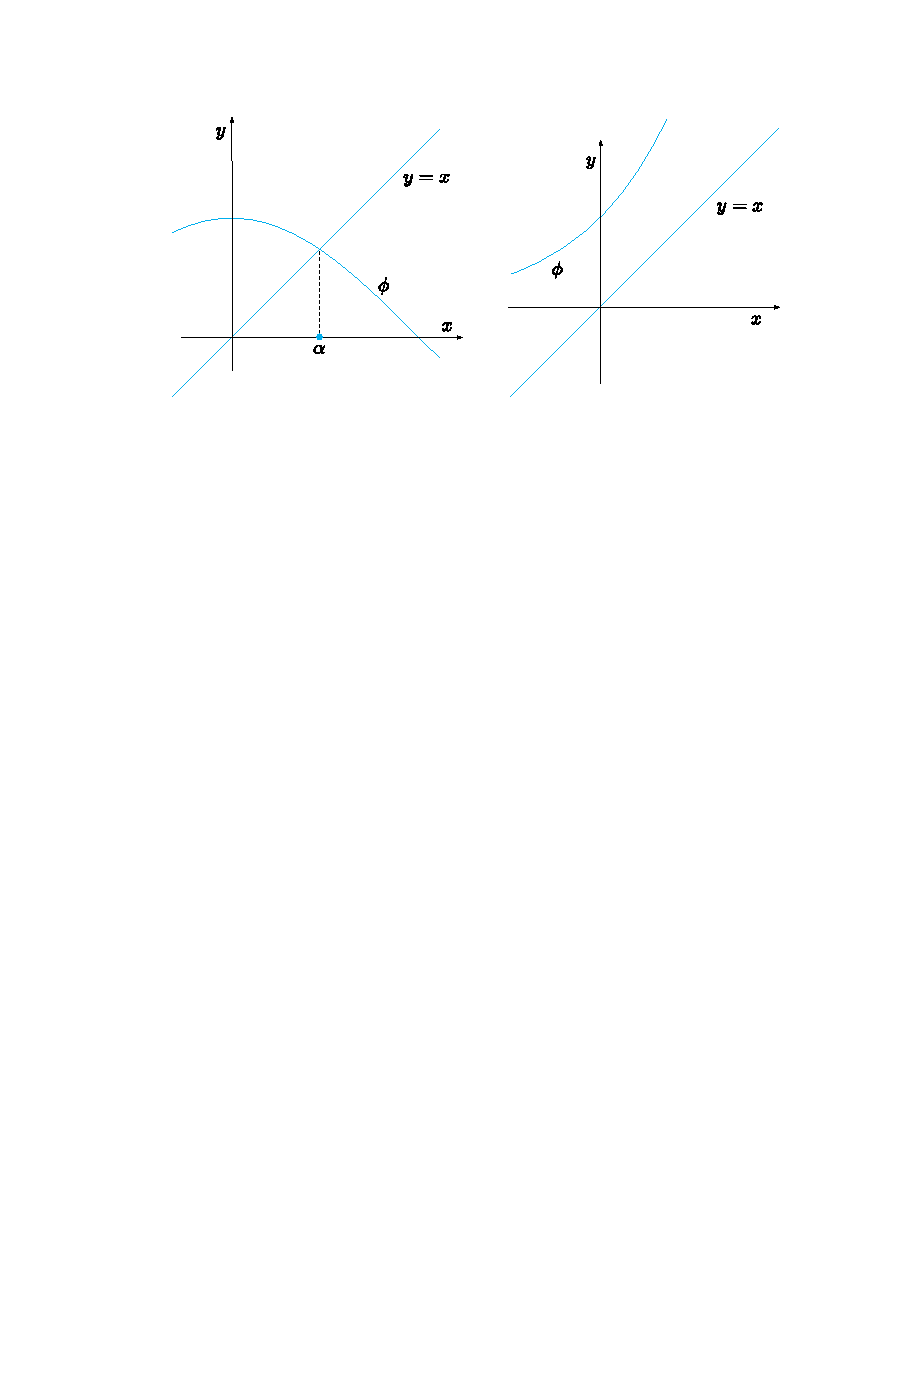
\includegraphics[width=\textwidth]{img/iterazioni-di-punto-fisso-1.pdf}
    \caption{La funzione $\phi\left(x\right) = \cos\left(x\right)$ (sx) ammette un solo punto fisso, mentre la funzione $\phi\left(x\right) = e^{x}$ (dx) non ne ammette alcuno.}
    \label{fig: non tutte le funzioni hanno un punto fisso}
\end{figure}

\hfill

\begin{figure}[!htp]
    \centering
    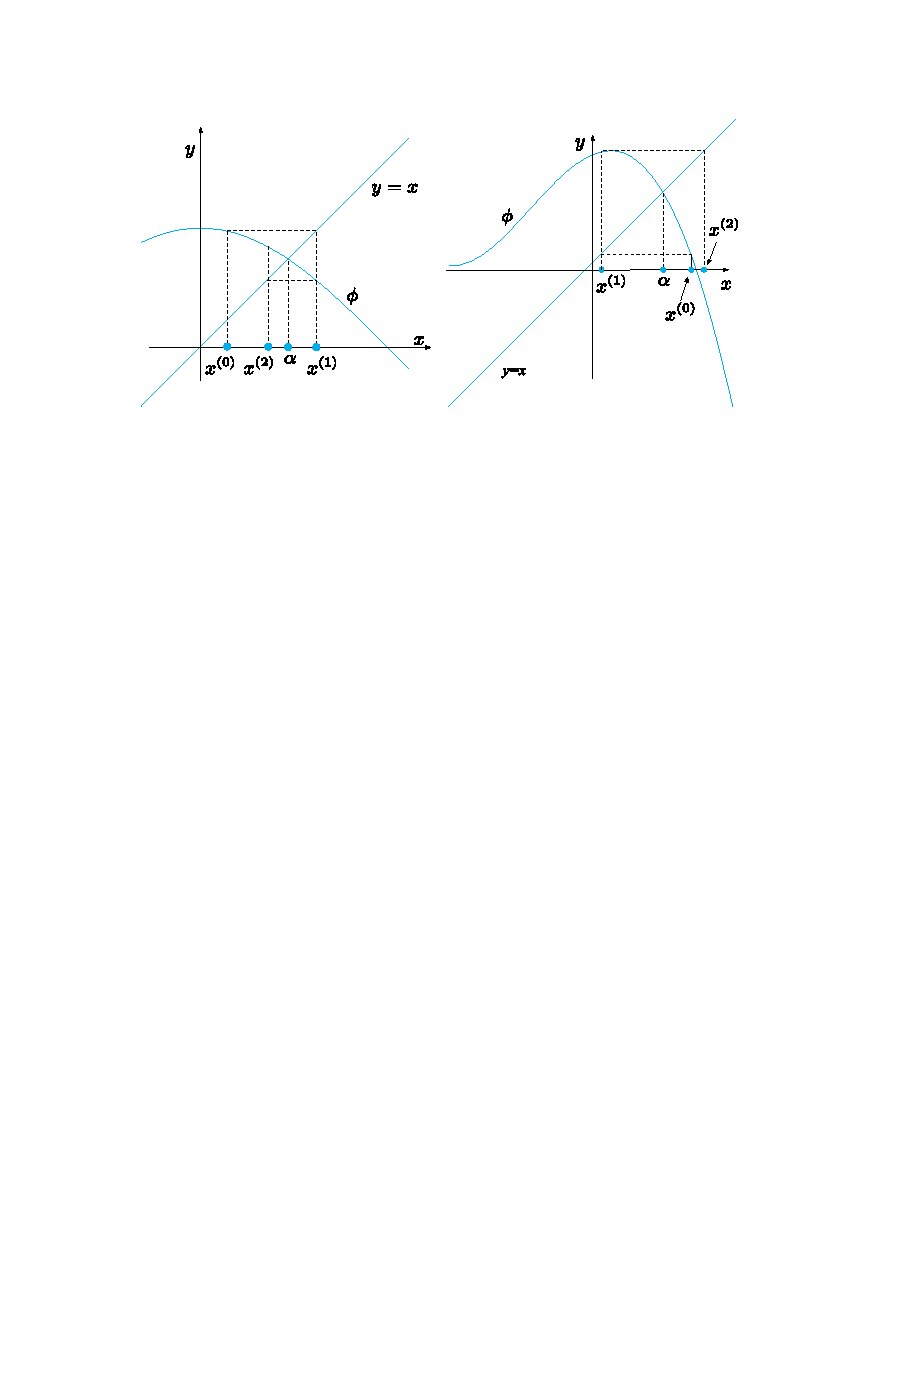
\includegraphics[width=\textwidth]{img/iterazioni-di-punto-fisso-2.pdf}
    \caption{Rappresentazione delle prime iterazioni di punto fisso per due funzioni di iterazione. Le iterazioni convergono verso il punto fisso $\alpha$ (sx), mentre si allontanano da $\alpha$ (dx).}
    \label{fig: interpretazione geometrica di un punto fisso}
\end{figure}

\newpage

\begin{definitionbox}[: quando una funzione ha un punto fisso?]
    Si consideri la successione (formula) \ref{eq: successione punto fisso} a pagina \pageref{eq: successione punto fisso}.
    \begin{enumerate}
        \item Si supponga che $\phi\left(x\right)$ sia continua nell'intervallo $\left[a,b\right]$ e che $\phi\left(x\right) \in \left[a,b\right]$ per ogni $x \in \left[a,b\right]$; allora \textbf{esiste almeno un punto fisso} $\alpha \in \left[a,b\right]$.

        \item Si supponga inoltre che esista un valore $L$ minore di $1$ tale per cui:
        \begin{equation*}
            \left|\phi\left(x_{1}\right)-\phi\left(x_{2}\right)\right| \le L \left|x_{1}-x_{2}\right|
        \end{equation*}
        Per ogni $x_{1},x_{2}$ appartenente all'insieme $\left[a,b\right]$. Con tale supposizione, allora $\phi$ ha un \textbf{unico punto fisso} $\phi\in\left[a,b\right]$ e la successione definita nell'equazione \ref{eq: successione punto fisso} a pagina \pageref{eq: successione punto fisso} converge a $\alpha$, qualunque sia il dato iniziale $x^{\left(0\right)}$ in $\left[a,b\right]$.

        La supposizione scritta in precedenza può essere riassunta in un'equazione:
        \begin{equation}
            \exists L < 1 \:\: t.c. \:\: \left| \phi\left(x_{1}\right)-\phi\left(x_{2}\right)\right| \le L \left|x_{1}-x_{2}\right| \hspace{1em} \forall x_{1},x_{2} \in \left[a,b\right]
        \end{equation}
    \end{enumerate}
\end{definitionbox}

\noindent
Nella pratica è però spesso \textbf{difficile delimitare a priori l'ampiezza dell'intervallo} $\left[a,b\right]$; in tal caso è utile il seguente risultato di convergenza locale:
\begin{theorem}[di Ostrowski]\index{teorema di Ostrowski}\label{theorem: teorema di Ostrowski}
    Sia $\alpha$ un punto fisso di una funzione $\phi$ continua e derivabile con continuità in un opportuno intorno $\mathcal{J}$ di $\alpha$. Se risulta $\left|\phi'\left(\alpha\right)\right| < 1$, allora esiste un $\delta > 0$ in corrispondenza del quale la successione $\left\{x^{\left(k\right)}\right\}$ converge ad $\alpha$, per ogni $x^{\left(0\right)}$ tale che $\left|x^{\left(0\right)} - \alpha \right| < \delta$. Inoltre si ha:
    \begin{equation}
        \displaystyle\lim_{k \rightarrow \infty} \dfrac{
            x^{\left(k+1\right)} - \alpha
        }{
            x^{\left(k\right)}-\alpha
        } = \phi'\left(\alpha\right)
    \end{equation}
\end{theorem}

\highspace
Dal teorema si deduce che le iterazioni di punto fisso convergono almeno linearmente cioè che, per $k$ sufficientemente grande, l'errore del passo $k+1$ si comporta come l'errore al passo $k$ moltiplicato per una costante, $\phi'\left(\alpha\right)$ nel teorema, indipendente da $k$ ed il cui valore assoluto è minore di $1$. Per questo motivo la costante viene chiamata \definition{fattore di convergenza} e la convergenza sarà tanto più rapida quanto più piccola è tale costante.

\begin{definitionbox}[: quando il metodo di punto fisso è convergente]
    Si suppongano valide le ipotesi del teorema di Ostrowski \ref{theorem: teorema di Ostrowski}. Se, inoltre, $\phi$ è derivabile con continuità due volte e se:
    \begin{equation*}
        \phi'\left(\alpha\right) = 0 \hspace{3em} \phi''\left(\alpha\right) \ne 0
    \end{equation*}
    Allora il metodo di punto fisso (eq. \ref{eq: successione punto fisso}) è convergente di ordine 2 e si ha:
    \begin{equation}
        \displaystyle\lim_{k \rightarrow \infty} \dfrac{
            x^{\left(k+1\right)} - \alpha
        }{
            \left(x^{\left(k\right)} - \alpha\right)^{2}
        } = \dfrac{1}{2}\phi''\left(\alpha\right)
    \end{equation}
\end{definitionbox}

\newpage

\noindent
Un'ultima osservazione interessante:
\begin{itemize}
    \item Nel caso in cui $\left| \phi'\left(\alpha\right) \right| > 1$, se $x^{\left(k\right)}$ è sufficientemente vicino ad $\alpha$, in modo tale che $\left| \phi'\left(x^{\left(k\right)}\right)\right| > 1$, allora $\left| \alpha - x^{\left(k+1\right)} \right| > \left| \alpha - x^{\left(k\right)} \right|$, e \textbf{non è possibile che la successione converga al punto fisso}.

    \item Nel caso in cui $\left| \phi'\left(\alpha\right) \right| = 1$ \textbf{non si può trarre alcuna conclusione} perché potrebbero verificarsi sia la convergenza sia la divergenza, a seconda delle caratteristiche della funzione di punto fisso.
\end{itemize}

    %%%%%%%%%%%%%%%%%%%%%%%%%%%%%%%%%%%%%%%%%%%%%%%%%%%%%%%
    % Metodi risolutivi per sistemi lineari e non lineari %
    %%%%%%%%%%%%%%%%%%%%%%%%%%%%%%%%%%%%%%%%%%%%%%%%%%%%%%%
    \section{Metodi risolutivi per sistemi lineari e non lineari}

\subsection{Metodi diretti per sistemi lineari}

\subsubsection{Metodo delle sostituzioni in avanti e all'indietro}

\begin{flushleft}
    \textcolor{Green3}{\faIcon{question-circle} \textbf{Perché sono importanti i metodi numerici?}}
\end{flushleft}
Si consideri il seguente \textbf{sistema lineare}:
\begin{equation*}
    Ax = b
\end{equation*}
Dove:
\begin{itemize}
    \item $A \in \mathbb{R}^{n \times n}$ di componenti $a_{ij}$ e $b \in \mathbb{R}^{n}$ sono valori noti.

    \item $x \in \mathbb{R}^{n}$ è il vettore delle incognite.
    
    \item La costante $n$ rappresenta il numero di equazioni lineari delle incognite $x_{j}$.
\end{itemize}
Con queste caratteristiche, è possibile rappresentare la $i$-esima equazione nel seguente modo:
\begin{equation*}
    \displaystyle\sum_{j=1}^{n} a_{ij} x_{j} = b_{i} \:\: \rightarrow \:\: a_{1i}x_{1} + a_{i2} x_{2} + \cdots + a_{in}x_{n} = b_{i} \hspace{2em} \forall i = 1, \dots , n
\end{equation*}
La \textbf{soluzione esatta} del sistema, chiamata \definition{formula di Cramer}, è:
\begin{equation}\label{eq: formula di Cramer}
    x_{j} = \dfrac{\det\left(A_{j}\right)}{\det\left(A\right)}
\end{equation}
Con $A_{j} = \left|a_{1} \:\: \dots \:\: a_{j-1} \:\: b \:\: a_{j+1} \:\: \dots \:\: a_{n} \right|$ e $a_{i}$ le colonne di $A$. Ovviamente la soluzione \textbf{esiste ed è unica se il determinante} della matrice $A$ è \textbf{diverso da zero}:
\begin{equation*}
    \det\left(A\right) \ne 0
\end{equation*}
Purtroppo questo metodo è \textbf{inutilizzabile} poiché il calcolo di un determinante richiede all'incirca $n!$ (fattoriale di $n$) operazioni.

\highspace
Risulta evidente che sia necessario uno studio approfondito di \textbf{metodi numerici che si traducano in algoritmi efficienti} da farli eseguire su calcolatori. Nelle seguenti pagine si introducono i primi due algoritmi \dquotes{efficienti}.

\newpage

\begin{definitionbox}
    Il seguente algoritmo rappresenta il \definition{metodo delle sostituzioni in avanti}.

    Dati:
    \begin{itemize}
        \item $L \in \mathbb{R}^{n \times n}$ matrice triangolare inferiore non singolare (cioè con determinante diverso da zero $\det\left(L\right) \ne 0$)
        
        \item $\mathbf{b} \in \mathbb{R}^{n}$ vettore termine noto
    \end{itemize}
    La soluzione è data da $Lx = \mathbf{b}$ con $x \in \mathbb{R}^{n}$. Più in generale si ha:
    \begin{equation}
        x_{i} = \dfrac{
            b_{i} - \displaystyle\sum_{j=1}^{i=1} L_{ij} \: x_{j}
        }{
            L_{ii}
        }
    \end{equation}
\end{definitionbox}

\noindent
Il \textbf{numero di operazioni} richieste dal metodo delle sostituzioni in avanti è dato da 1 sottrazione, $i-1$ moltiplicazioni, $i-2$ addizioni e 1 divisione:
\begin{equation}
    \# op. = \displaystyle\sum_{i=1}^{n} \left(i-1\right) + \left(i-2\right) + 1 + 1 = \sum_{i=1}^{n} \left(2i-1\right) = n^{2}
\end{equation}
Per completezza si presenta anche il metodo delle sostituzioni all'indietro.

\begin{definitionbox}
    Il seguente algoritmo rappresenta il \definition{metodo delle sostituzioni all'indietro}.

    Dati:
    \begin{itemize}
        \item $U \in \mathbb{R}^{n \times n}$ matrice triangolare superiore non singolare (cioè con determinante diverso da zero $\det\left(U\right) \ne 0$)
        
        \item $\mathbf{b} \in \mathbb{R}^{n}$ vettore termine noto
    \end{itemize}
    La soluzione è data da $Ux = \mathbf{b}$ con $x \in \mathbb{R}^{n}$. Più in generale si ha:
    \begin{equation}
        x_{i} = \dfrac{
            b_{i} - \displaystyle\sum_{j=1}^{i=1} U_{ij} \: x_{j}
        }{
            U_{ii}
        }
    \end{equation}
\end{definitionbox}

\noindent
Il numero di operazioni è il medesimo del metodo delle sostituzioni in avanti.
    \subsection{Metodi iterativi per sistemi lineari}
    \subsection{Metodi numerici per sistemi non lineari}
    
    %%%%%%%%%%%%%%%
    % Laboratorio %
    %%%%%%%%%%%%%%%
    \section{Laboratorio}

\subsection{Introduzione al linguaggio MATLAB}

L'introduzione al linguaggio di programmazione MATLAB sarà molto rapido. Si assume dunque che l'interfaccia grafica sia familiare e che concetti base di programmazione (per esempio \dquotes{che cos'è una variabile?}) siano ben noti.

\highspace
In MATLAB, l'assegnazione di scalari a delle variabili è classica, quindi si utilizza il simbolo uguale: \texttt{a = 1} (assegnazione del valore \texttt{1} alla variabile \texttt{a}). Inoltre, il linguaggio è \emph{case sensitive}, di conseguenza la variabile \texttt{a} è diversa dalla variabile \texttt{A}. Alcuni comandi utili e generali:
\begin{itemize}
    \item \texttt{help \emph{nome-comando}}, per avere informazioni in più riguardo al comando \texttt{\emph{nome-comando}};

    \item \texttt{clear \emph{nome-variabile}}, per rimuovere la variabile \texttt{\emph{nome-variabile}} dalla memoria. Se non viene inserito il \texttt{\emph{nome-variabile}}, vengono rimosse tutte le variabili dalla memoria.

    \item \texttt{who}, per visualizzare le variabili attualmente in memoria.

    \item \texttt{clc}, per ripulire la \emph{Command Window}.
\end{itemize}

\begin{table}[!htp]
    \centering
    \begin{tabular}{@{} p{21em} l @{}}
        \toprule
        \textbf{Argomento} & \textbf{Pagina} \\
        \midrule
        Well-known variables    & Pag. \hyperlink{
            lab: Well-known variables
        }{
            \hypergetpageref{lab: Well-known variables}
        } \\
        Cambiare il formato delle variabili: \texttt{format} & Pag. 
        \hyperlink{
            lab: Cambiare il formato delle variabili: format
        }{
            \hypergetpageref{lab: Cambiare il formato delle variabili: format}
        } \\
        Assegnamento di vettori e matrici & Pag. 
        \hyperlink{
            lab: Assegnamento di vettori e matrici
        }{
            \hypergetpageref{lab: Assegnamento di vettori e matrici}
        } \\
        Operazioni su vettori e matrici & Pag. \hyperlink{
            lab: Operazioni su vettori e matrici
        }{
            \hypergetpageref{lab: Operazioni su vettori e matrici}
        } \\
        Funzioni intrinseche per vettori e matrici & Pag. \hyperlink{
            lab: Funzioni intrinseche per vettori e matrici
        }{
            \hypergetpageref{lab: Funzioni intrinseche per vettori e matrici}
        } \\
        Funzioni matematiche elementari & Pag. \hyperlink{
            lab: Funzioni matematiche elementari
        }{
            \hypergetpageref{lab: Funzioni matematiche elementari}
        } \\
        Funzioni per definire vettori o matrici particolari & Pag. \hyperlink{
            lab: Funzioni per definire vettori o matrici particolari
        }{
            \hypergetpageref{lab: Funzioni per definire vettori o matrici particolari}
        } \\
        \bottomrule
    \end{tabular}
    \caption{Argomenti trattati.}
\end{table}

\begin{flushleft}
    \large
    \hypertarget{
        lab: Well-known variables
    }{
        \textcolor{Red3}{\textbf{Well-known variables}}
    }
    \label{lab: Well-known variables}
\end{flushleft}
Esistono alcune variabili che sono ben note e hanno valori prestabiliti. Tra le più importanti:
\begin{itemize}
    \item \texttt{pi}, che rappresenta il $\pi$ e MATLAB gli assegna il valore \texttt{3.1416}
    
    \item \texttt{i}, che rappresenta l'unità immaginaria e MATLAB gli assegna il valore \texttt{0.0000 + 1.0000i}
    
    \item \texttt{eps}, che rappresenta il più piccolo valore rappresentabile nel calcolatore (PC) attualmente in uso. Solitamente, \texttt{eps} ritorna il valore \texttt{2.2204e-16}.
\end{itemize}
Questo tipo di variabili possono essere ridefinite, ma \underline{non} è una \emph{good practice}.

\newpage

\begin{flushleft}
    \large
    \hypertarget{
        lab: Cambiare il formato delle variabili: format
    }{
        \textcolor{Red3}{\textbf{Cambiare il formato delle variabili: \texttt{format}}}
    }
    \label{lab: Cambiare il formato delle variabili: format}
\end{flushleft}
Il comando \texttt{format} è utilizzato per cambiare il formato con cui sono rappresentate le variabili. MATLAB \underline{non} cambia la precisione della variabile (quindi non si ottiene una precisione maggiore dopo la virgola), ma modifica soltanto la rappresentazione. Di default MATLAB utilizza una rappresentazione di tipo \texttt{short}. Tra i più utilizzati (di default \texttt{pi} è uguale a \texttt{3.1416}):
\begin{itemize}
    \item \texttt{default} per reimpostare la rappresentazione di default.

    \item Decimale:
    \begin{itemize}
        \item \texttt{short}, rappresentazione a 5 cifre:
        \lstinputlisting[language=MATLAB]{code/introduzione-al-linguaggio-MATLAB/short.m}

        \item \texttt{long}, rappresentazione a 15 cifre:
        \lstinputlisting[language=MATLAB]{code/introduzione-al-linguaggio-MATLAB/long.m}
    \end{itemize}

    \item \emph{Floating point}:
    \begin{itemize}
        \item \texttt{short e}, rappresentazione a 5 cifre floating point:
        \lstinputlisting[language=MATLAB]{code/introduzione-al-linguaggio-MATLAB/short-floating-point.m}

        \item \texttt{long e}, rappresentazione a 15 cifre floating point:
        \lstinputlisting[language=MATLAB]{code/introduzione-al-linguaggio-MATLAB/long-floating-point.m}
    \end{itemize}
\end{itemize}
Altri formati si possono trovare nella \href{https://uk.mathworks.com/help/releases/R2024a/matlab/ref/format.html#btiwmh5-1-style}{documentazione ufficiale}.

\newpage

\begin{flushleft}
    \large
    \hypertarget{
        lab: Assegnamento di vettori e matrici
    }{
        \textcolor{Red3}{\textbf{Assegnamento di vettori e matrici}}
    }
    \label{lab: Assegnamento di vettori e matrici}
\end{flushleft}
\begin{itemize}
    \item \textbf{Vettore riga}, si può creare utilizzando uno spazio tra i valori o una virgola \texttt{,}:
    \lstinputlisting[language=MATLAB]{code/introduzione-al-linguaggio-MATLAB/vettori-1.m}

    \item \textbf{Vettore colonna}, si crea usando il punto e virgola \texttt{;}:
    \lstinputlisting[language=MATLAB]{code/introduzione-al-linguaggio-MATLAB/vettori-2.m}
\end{itemize}
Talvolta può essere utile la generazione automatica di un vettore riga (sono ammessi anche i valori negativi e con la virgola ovviamente):
\begin{itemize}
    \item \textbf{Vettore riga generato linearmente}, si crea usando i due punti e specificando il valore di inizio e il valore di fine:
    \lstinputlisting[language=MATLAB]{code/introduzione-al-linguaggio-MATLAB/vettori-3.m}

    \item \textbf{Vettore riga generato usando un passo}, si crea usando i due punti e specificando (in ordine) il valore di inizio, il \dquotes{salto}, e il valore di fine. Nel caso in cui il salto sia troppo grande e si superi il valore di fine, MATLAB prenderà il primo valore ammissibile:
    \lstinputlisting[language=MATLAB]{code/introduzione-al-linguaggio-MATLAB/vettori-4.m}

    \item \textbf{Vettore riga generato con valori uniformemente distanziati}, si crea usando la funzione \texttt{linspace}, la quale accetta tre parametri:
    \begin{itemize}
        \item \texttt{x1}, valore di partenza.
        \item \texttt{x2}, valore di fine.
        \item \texttt{n}, numero di valori da generare; se non specificato, di default è \texttt{100}; se il valore inserito è zero o minore, viene creato un vettore vuoto.
    \end{itemize}
    \lstinputlisting[language=MATLAB]{code/introduzione-al-linguaggio-MATLAB/vettori-5.m}
\end{itemize}
Le matrici possono essere create a mano o usando la combinazione delle tecniche viste in precedenza:
\begin{itemize}
    \item \textbf{Matrice}, le righe si creano usando gli spazi e le colonne si creano usando il punto e virgola:
    \lstinputlisting[language=MATLAB]{code/introduzione-al-linguaggio-MATLAB/matrici-1.m}

    \item \textbf{Matrice creata usando la generazione lineare dei vettori}, si possono utilizzare le tecniche precedenti e i punti e virgola:
    \lstinputlisting[language=MATLAB]{code/introduzione-al-linguaggio-MATLAB/matrici-2.m}
\end{itemize}

\newpage

\begin{flushleft}
    \large
    \hypertarget{
        lab: Operazioni su vettori e matrici
    }{
        \textcolor{Red3}{\textbf{Operazioni su vettori e matrici}}
    }
    \label{lab: Operazioni su vettori e matrici}
\end{flushleft}
\begin{itemize}
    \item \textbf{Trasposizione}, la classica operazione eseguita con le matrici o vettori, si esegue con la keyword \texttt{'} oppure usando la funzione \texttt{transpose}:
    \lstinputlisting[language=MATLAB]{code/introduzione-al-linguaggio-MATLAB/operazioni-vettori-matrici-1.m}

    \item \textbf{Somma e sottrazione}
    \begin{itemize}
        \item Tra \textbf{vettore e scalare}:
        \lstinputlisting[language=MATLAB]{code/introduzione-al-linguaggio-MATLAB/operazioni-vettori-matrici-2.m}

        \item Tra \textbf{vettore e matrice}:
        \lstinputlisting[language=MATLAB]{code/introduzione-al-linguaggio-MATLAB/operazioni-vettori-matrici-3.m}

        \item Tra \textbf{matrice e scalare}:
        \lstinputlisting[language=MATLAB]{code/introduzione-al-linguaggio-MATLAB/operazioni-vettori-matrici-4.m}

        \item Tra \textbf{matrice e matrice}:
        \lstinputlisting[language=MATLAB]{code/introduzione-al-linguaggio-MATLAB/operazioni-vettori-matrici-5.m}
    \end{itemize}

    \item \textbf{Prodotto}
    \begin{itemize}
        \item \textbf{Prodotto matriciale}:
        \lstinputlisting[language=MATLAB]{code/introduzione-al-linguaggio-MATLAB/operazioni-vettori-matrici-6.m}

        \item \textbf{Prodotto punto per punto}, in MATLAB è possibile moltiplicare ogni cella di una matrice (o vettore) per la corrispettiva cella della matrice (o vettore) moltiplicata. La keyword utilizzata è \texttt{.*}:
        \lstinputlisting[language=MATLAB]{code/introduzione-al-linguaggio-MATLAB/operazioni-vettori-matrici-7.m}
    \end{itemize}

    \item \textbf{Potenza}
    \begin{itemize}
        \item \textbf{Potenza matriciale}:
        \lstinputlisting[language=MATLAB]{code/introduzione-al-linguaggio-MATLAB/operazioni-vettori-matrici-8.m}

        \item \textbf{Potenza punto per punto}, come per il prodotto, è possibile elevare al quadrato ogni valore della matrice (o vettore):
        \lstinputlisting[language=MATLAB]{code/introduzione-al-linguaggio-MATLAB/operazioni-vettori-matrici-9.m}
    \end{itemize}
\end{itemize}

\newpage

\begin{flushleft}
    \large
    \hypertarget{
        lab: Funzioni intrinseche per vettori e matrici
    }{
        \textcolor{Red3}{\textbf{Funzioni intrinseche per vettori e matrici}}
    }
    \label{lab: Funzioni intrinseche per vettori e matrici}
\end{flushleft}
Qua di seguito si elencano le funzioni più importanti da utilizzare per i vettori e le matrici.
\begin{itemize}
    \item \texttt{\textbf{size}}, restituisce la dimensione del vettore o della matrice nel formato \texttt{\emph{righe} \emph{colonne}}. Specificando anche un valore (o vettore) come parametro, la funzione restituisce la dimensione (un vettore contenente le dimensioni richieste) nella \dquotes{dimensione} richiesta:
    \lstinputlisting[language=MATLAB]{code/introduzione-al-linguaggio-MATLAB/operazioni-vettori-matrici-10.m}

    \item \texttt{\textbf{length}}, restituisce la lunghezza del vettore e per le matrici restituisce il numero degli elementi per ogni riga:
    \lstinputlisting[language=MATLAB]{code/introduzione-al-linguaggio-MATLAB/operazioni-vettori-matrici-11.m}

    \item \texttt{\textbf{max}}, \texttt{\textbf{min}}, calcolano rispettivamente il massimo e il minimo valore delle componenti di un vettore; per le matrici viene presa in considerazione ogni colonna e calcolato il massimo o minimo:
    \lstinputlisting[language=MATLAB]{code/introduzione-al-linguaggio-MATLAB/operazioni-vettori-matrici-12.m}

    \item \texttt{\textbf{sum}}, \texttt{\textbf{prod}}, calcola rispettivamente la somma e il prodotto degli elementi che compongono il vettore; nel caso di una matrice, viene presa in considerazione ogni colonna e calcolata la somma o il prodotto. Inoltre, i due comandi possono prendere un argomento in più per eseguire il calcolo in una dimensione specifica (cosa sensata con le matrici):
    \lstinputlisting[language=MATLAB]{code/introduzione-al-linguaggio-MATLAB/operazioni-vettori-matrici-13.m}

    \item \texttt{\textbf{norm}}, la norma di un vettore o di una matrice. Passando un vettore o un matrice, viene calcolata di default la norma euclidea (norma 2):
    \begin{equation*}
        \left|\left| \mathrm{v} \right|\right|_{2} = \sqrt{\sum_{i = 2}^{\texttt{length(v)} \mathrm{v}_{i}^{2}}}
    \end{equation*}
    Passando un valore aggiuntivo, esso rappresenterà l'ordine della norma:
    \begin{equation*}
        \left|\left| \mathrm{v} \right|\right|_{n} = \left( \sum_{i = 2}^{\texttt{length(v)} \left| \mathrm{v}_{i} \right|^{n}} \right)^{\frac{1}{n}}
    \end{equation*}
    Infine, con \texttt{inf} viene calcolata la norma infinito:
    \begin{equation*}
        \left|\left| \mathrm{v} \right|\right|_{\infty} = \underset{1 \le i \le \texttt{length(v)}}{\max} \left| \mathrm{v}_{i} \right|
    \end{equation*}
    \lstinputlisting[language=MATLAB]{code/introduzione-al-linguaggio-MATLAB/operazioni-vettori-matrici-14.m}

    \item \texttt{\textbf{abs}}, rappresenta il valore assoluto e restituisce il vettore o matrice dopo aver applicato il valore assoluto a ciascun elemento:
    \lstinputlisting[language=MATLAB]{code/introduzione-al-linguaggio-MATLAB/operazioni-vettori-matrici-15.m}

    \newpage

    \item \texttt{\textbf{diag}}, estrae la diagonale di una matrice esistente, oppure ne crea una con i valori dati come input. Inoltre, può creare una matrice con la diagonale spostata a seconda del valore dato (si veda l'esempio):
    \lstinputlisting[language=MATLAB]{code/introduzione-al-linguaggio-MATLAB/operazioni-vettori-matrici-16.m}
\end{itemize}

\newpage

\begin{flushleft}
    \large
    \hypertarget{
        lab: Funzioni matematiche elementari
    }{
        \textcolor{Red3}{\textbf{Funzioni matematiche elementari}}
    }
    \label{lab: Funzioni matematiche elementari}
\end{flushleft}
Qua di seguito una lista di alcune funzioni matematiche elementari. Gli esempi e la sintassi non verranno mostrati poiché è sempre la medesima:
\begin{equation*}
    \texttt{\emph{funzione}(\emph{parametro})}
\end{equation*}
\begin{table}[!htp]
    \centering
    \begin{tabular}{@{} l l @{}}
        \toprule
        \textbf{Funzione} & \textbf{Comando} \\
        \midrule
        \textbf{Radice quadrata}                & \texttt{sqrt} \\
        \textbf{Esponenziale}                   & \texttt{exp} \\
        \textbf{Logaritmo Naturale}             & \texttt{log} \\
        \textbf{Logaritmo In Base \texttt{2}}   & \texttt{log2} \\
        \textbf{Logaritmo In Base \texttt{10}}  & \texttt{log10} \\
        \textbf{Seno}                           & \texttt{sin} \\
        \textbf{Arcoseno}                       & \texttt{asin} \\
        \textbf{Coseno}                         & \texttt{cos} \\
        \textbf{Arcocoseno}                     & \texttt{acos} \\
        \textbf{Tangente}                       & \texttt{tan} \\
        \bottomrule
    \end{tabular}
    \caption{Funzioni matematiche elementari.}
\end{table}

\longline

\begin{flushleft}
    \large
    \textcolor{Red3}{\textbf{Iterazione con il ciclo for}}
\end{flushleft}
In MATLAB il ciclo for viene eseguito con la seguente sintassi.
\lstinputlisting[language=MATLAB]{code/introduzione-al-linguaggio-MATLAB/for-1.m}
Di seguito si riporta un ciclo \texttt{for} che itera sulla diagonale secondaria di una matrice:
\lstinputlisting[language=MATLAB]{code/introduzione-al-linguaggio-MATLAB/for-2.m}

\newpage

\begin{flushleft}
    \large
    \hypertarget{
        lab: Funzioni per definire vettori o matrici particolari
    }{
        \textcolor{Red3}{\textbf{Funzioni per definire vettori o matrici particolari}}
    }
    \label{lab: Funzioni per definire vettori o matrici particolari}
\end{flushleft}
In queste pagine vengono presentate alcuni funzioni utili che consentono di creare matrici o vettori \dquotes{particolari}.
\begin{itemize}
    \item \textbf{Vettore/Matrice nulla}, con la funzione \texttt{zeros} è possibile creare una matrice o un vettore di tutti zeri. I parametri ammessi corrispondono alla dimensione del vettore o matrice:
    \lstinputlisting[language=MATLAB]{code/introduzione-al-linguaggio-MATLAB/vettori-matrici-particolari-1.m}

    \item \textbf{Vettore unario/Matrice unaria}, con la funzione \texttt{ones} è possibile creare una matrice o un vettore di tutti uni. I parametri ammessi corrispondono alla dimensione del vettore o matrice:
    \lstinputlisting[language=MATLAB]{code/introduzione-al-linguaggio-MATLAB/vettori-matrici-particolari-2.m}

    \newpage

    \item \textbf{Matrice identità}, con la funzione \texttt{eye} è possibile creare una matrice identità. I parametri ammessi corrispondono alla dimensione del vettore o matrice:
    \lstinputlisting[language=MATLAB]{code/introduzione-al-linguaggio-MATLAB/vettori-matrici-particolari-3.m}

    \item \textbf{Matrice/Vettore riga di numeri casuali interi e non}, con il comando \texttt{rand} si genera una matrice di numeri casuali nell'intervallo $\left[0,1\right]$ con la virgola, mentre con il comando \texttt{randi} si genera una matrice di numeri casuali interi (primo parametro deve essere specificato il range dei valori):
    \lstinputlisting[language=MATLAB]{code/introduzione-al-linguaggio-MATLAB/vettori-matrici-particolari-4.m}
\end{itemize}

\newpage

\subsubsection{Esercizio}

Creare una funzione (file) chiamato \texttt{mat\_hilbert.m} che fornisca la matrice di Hilbert avente una generica dimensione \texttt{n}. Ogni cella della matrice di Hilbert deve rispettare la seguente condizione:
\begin{equation*}
    a_{ij} = \dfrac{1}{i + j - 1}
\end{equation*}
Dopo aver creato la funzione, utilizzare la funzione nativa di MATLAB \texttt{hilb}, per verificare il risultato ottenuto.

\begin{flushleft}
    \textcolor{Green4}{\textbf{Soluzione}}
\end{flushleft}
Il codice non ha bisogno di grandi spiegazioni. Vi è un controllo iniziale per verificare l'argomento inserito dall'utente e successivamente due cicli \texttt{for} per popolare la matrice:
\lstinputlisting[language=MATLAB]{code/introduzione-al-linguaggio-MATLAB/mat_hilbert.m}
Il risultato:
\lstinputlisting[language=MATLAB]{code/introduzione-al-linguaggio-MATLAB/mat_hilbert-res.m}    
    \subsection{Zeri di funzione}

\subsubsection{Grafici di funzione}

In MATLAB una funzione $f\left(x\right)$ viene memorizzata come un vettore. In particolare, il vettore $y$ ottenuto valutando $f$ nel vettore delle ascisse $x$. Per cui la rappresentazione della funzione $f\left(x\right)$ è di fatto la rappresentazione del vettore $y$ contro il vettore $x$.

\highspace
Per introdurre i concetti di funzione e grafici di funzione, si presentano qua di seguito alcuni esempi di caso d'uso.

\highspace
\example{\emph{Definire le seguenti variabili:
\begin{itemize}
    \item $x$: vettore di estremi $0$ e $10$ con passo $0.1$
    \item $y = e^{x} + 1$
\end{itemize}}}

\noindent
Il vettore delle ascisse $x$ può essere costruito banalmente con il seguente costrutto:
\begin{lstlisting}[language=MATLAB]
x = [0 : 0.1 : 10];\end{lstlisting}
Per quanto riguarda la \textbf{funzione}, si utilizza la keyword \texttt{\@} per indicare che $f$ ha come input un valore (\texttt{x}) e rappresenta la funzione \texttt{exp(x)+1}. In questo caso, la funzione si dice anonima. Per dichiarare funzioni esplicite, si rimanda alla \href{https://it.mathworks.com/help/releases/R2024a/matlab/ref/function_handle.html}{documentazione ufficiale}.
\begin{lstlisting}[language=MATLAB]
f = @(x) exp(x) + 1\end{lstlisting}
Una volta definita una \textbf{funzione}, per \textbf{valutarla in uno o più punti}, si utilizzerà banalmente la sintassi matematica:
\begin{lstlisting}[language=MATLAB]
f(2)

ans =

    8.3891

f(0:3)

ans =

    2.0000    3.7183    8.3891   21.0855\end{lstlisting}
Da notare che se l'argomento è un vettore, allora il risultato sarà un vettore della medesima lunghezza del vettore dato in input.

\newpage

\noindent
\example{\emph{Utilizzando le variabili precedentemente definite, disegnare il grafico della funzione $y = e^{x} + 1$ nell'intervallo $\left[0, 10\right]$.}}

\highspace
Per disegnare il grafico si utilizza il comando \texttt{plot}. Di default questa funzione disegna i valori in un piano cartesiano usando segmenti rettilinei (retta spezzata):
\begin{lstlisting}[language=MATLAB]
y = f(x);
plot(x, y)\end{lstlisting}
\begin{figure}[!htp]
    \centering
    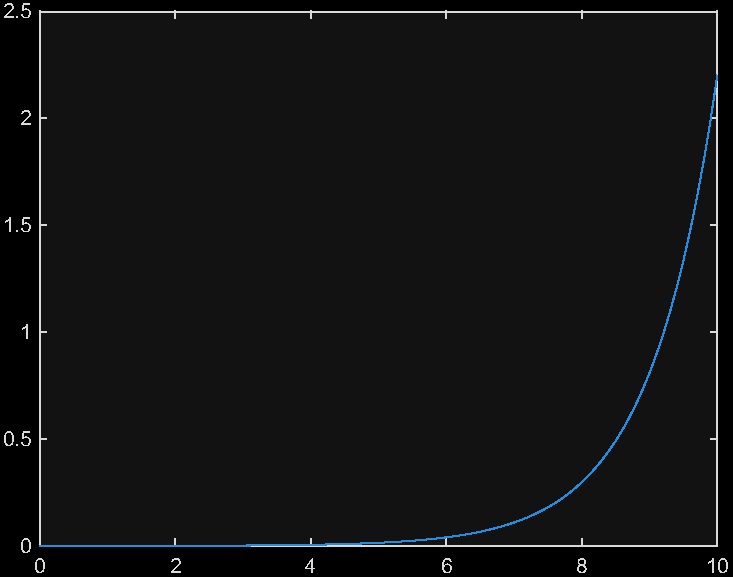
\includegraphics[width=.6\textwidth]{img/grafici-di-funzione-1.pdf}
\end{figure}

\noindent
Per evitare che MATLAB sovrascriva la figura nella finestra aperta, è possibile numerarle usando la funzione \texttt{figure} (e.g. \texttt{figure(1); plot(x,y); figure(2); plot(0:3, 0:3)}).

\highspace
La funzione \texttt{plot} accetta determinati valori per modificare il grafico finale. Nella \href{https://it.mathworks.com/help/releases/R2024a/matlab/ref/plot.html}{documentazione ufficiale} è possibile trovare l'intera lista e alcuni esempi. Scrivendo \texttt{plot(x, f(x), 'linewidth', 2)}, il parametro \texttt{'linewidth'} consente di definire lo spessore delle curve. Il valore che viene specificato in questo caso è \texttt{2} e il risultato:
\begin{figure}[!htp]
    \centering
    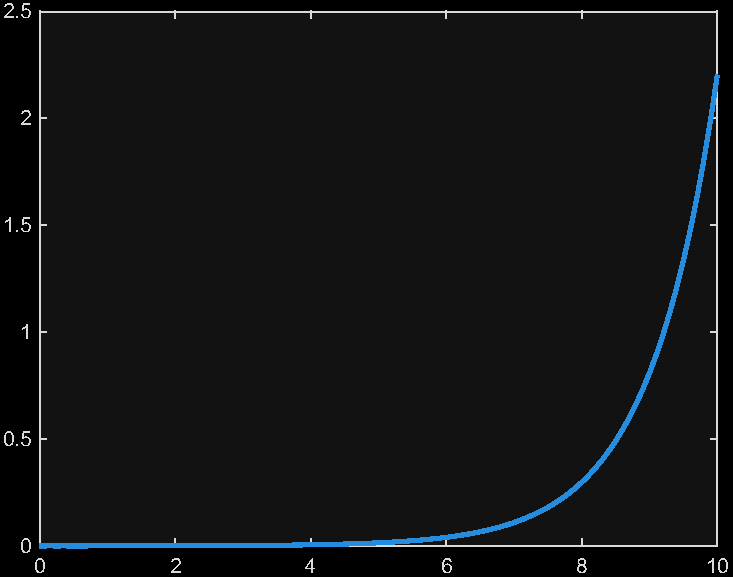
\includegraphics[width=.6\textwidth]{img/grafici-di-funzione-2.pdf}
\end{figure}

\newpage

\noindent
Usando il comando \texttt{hold on} per fare un confronto tra i vari grafici e invocando di nuovo la funzione \texttt{plot} ma con parametri differenti, si ottiene:
\begin{lstlisting}[language=MATLAB]
figure(1)
plot(x, f(x), 'linewidth', 2)
hold on
plot(x, -f(x), 'r', 'linewidth', 2)\end{lstlisting}

\begin{figure}[!htp]
    \centering
    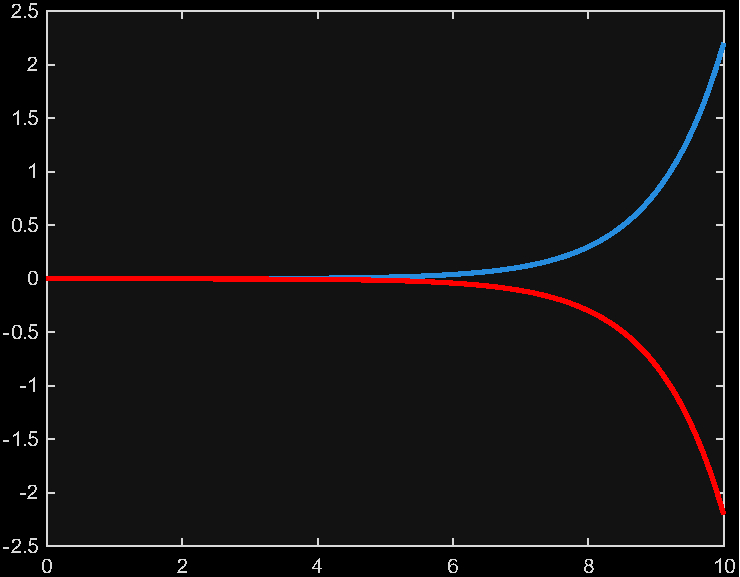
\includegraphics[width=.6\textwidth]{img/grafici-di-funzione-3.pdf}
\end{figure}

\noindent
\example{\emph{Disegnare il grafico in scala semi-logaritmica (logaritmica solo per le ordinate) della funzione $y = e^{x}$ nell'intervallo $\left[0, 10\right]$. È possibile prevedere come sarà il grafico in scala semi-logaritmica della funzione $y=e^{2x}$? Verificare la risposta tracciando sulla medesima finestra le due funzioni utilizzando colori diversi per i due grafici.}}

\highspace
Per disegnare il grafico in scala semi-logaritmica (logaritmica sulle ordinate) si utilizza il comando \texttt{semilogy} e si aggiunge anche la griglia:
\begin{lstlisting}[language=MATLAB]
semilogy(x, exp(x), 'linewidth', 2)
grid on\end{lstlisting}
\begin{figure}[!htp]
    \centering
    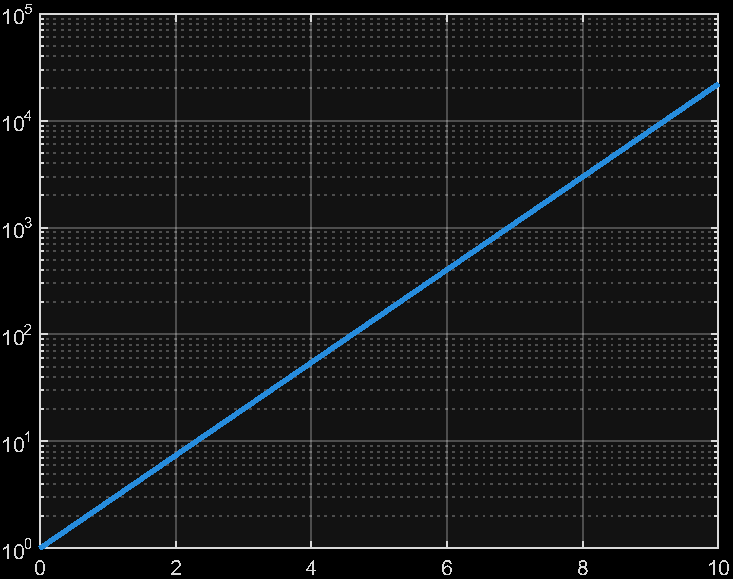
\includegraphics[width=.6\textwidth]{img/grafici-di-funzione-4.pdf}
    \caption*{È una retta poiché $\log_{10}\left(y\right) = \log_{10}\left(e^{x}\right) = x\log_{10}\left(e\right)$.}
\end{figure}

\begin{itemize}
    \item Il comando \texttt{semilogy} è l'equivalente di \texttt{plot} ma traccia un \textbf{grafico con l'asse delle ordinate in scala logaritmica}.

    \item Il comando \texttt{semilogx} traccia un \textbf{grafico con l'asse delle ascisse logaritmico}.
    
    \item Il comando \texttt{loglog} traccia un grafico in cui entrambi gli assi sono in scala logaritmica.
\end{itemize}
Passando alla risoluzione dell'esercizio, dato che $\log_{10}\left(e^{2x}\right) = 2x\log_{10}\left(e\right)$, disegnando in scala semi-logaritmica la funzione $y = e^{2x}$, si otterrà una retta con pendenza doppia rispetto alla retta precedentemente disegnata.
\begin{lstlisting}[language=MATLAB]
hold on
semilogy(x, exp(2 * x), 'r', 'linewidth', 2)
% oppure in un solo comando senza usare hold on
% semilogy(x, exp(x), 'b', x, exp(2*x), 'r', 'linewidth', 2)
title('Grafico di exp(x) e di exp(2x)')
xlabel('Scala lineare')
ylabel('Scala logaritmica')
grid on
legend('exp(x)', 'exp(2*x)', 'Location', 'NorthWest')\end{lstlisting}
\begin{figure}[!htp]
    \centering
    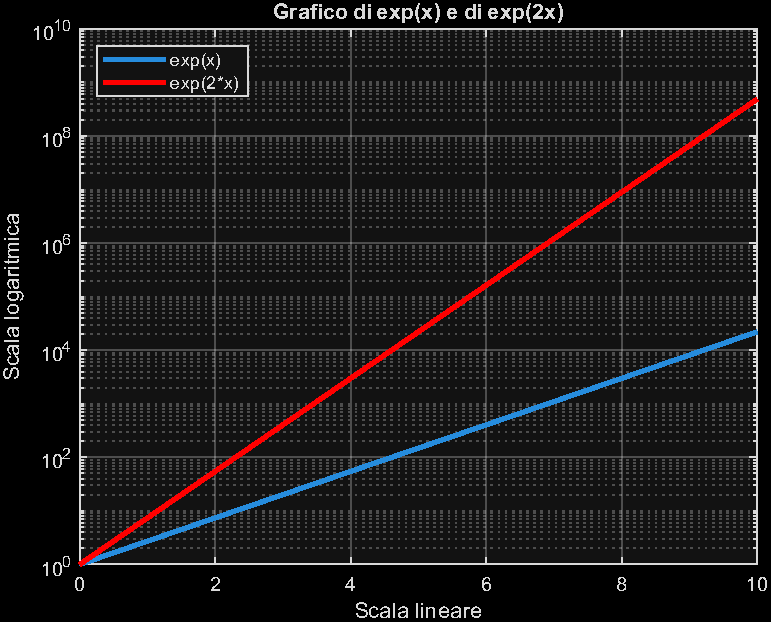
\includegraphics[width=.7\textwidth]{img/grafici-di-funzione-5.pdf}
\end{figure}

\noindent
Il comando \texttt{legend} attribuisce alle curve disegnate da \texttt{plot} le stringhe di testo che gli vengono passate. Attenzione che alcune stringhe, come \texttt{'Location'} e \texttt{'NorthWest'}, vengono interpretate dalla funzione come comandi veri e propri. In questo caso si chiede di inserire una legenda in alto a sinistra.

    %%%%%%%%%%%%%%%%%%%%%%%%%%
    % Bibliography and index %
    %%%%%%%%%%%%%%%%%%%%%%%%%%
    \bibliography{bibtex}{}
\bibliographystyle{plain}

\newpage

\printindex
\end{document}